\section{Classical cryptography} \label{classical-cryptography}

There are several cryptographic primitives that are essential building blocks for the information security protocols we all rely upon \cite{bib:Schneier96}.

\subsection{Private-key
cryptography} \label{private-key-cryptography}

Private key cryptography refers to encryption where the same key is used for both encryption and decryption, a property that has led to such schemes also being referred to as \emph{symmetric} ciphers.

For a given message $m$, key $k$ and ciphertext $c$, the encryption and decryption operators satisfy the properties,
\begin{align}
	{\tt enc}_k(m) &\to c, \nonumber\\
	{\tt dec}_k(c) &\to m, \nonumber\\
	{\tt dec}_k \circ {\tt enc}_k(m) &= m, 
\end{align}
where $\circ$ denotes operator composition.

Modern private-key cryptographic standards, such as AES-256, are considered but not proven to be safe against future quantum computers as they are not believed to exhibit any inherent mathematical structures that quantum computers can efficiently exploit. They additionally have the advantage of being algorithmically very fast, and do not incur any overhead in encrypted message size --- plaintexts and ciphertexts are typically of the same size. This is in contrast to public key cryptography, where ciphertexts are significantly larger than plaintexts.

Despite these advantages symmetric ciphers are not very practical to utilise in isolation as they require secrecy when exchanging secret keys for future use. When communicating with someone a long distance away who we aren't able to meet in a dark back alley, this becomes impractical, requiring public-key cryptography for the purposes of key exchange.

Block and stream ciphers are optimal for different use cases. For example, when dealing with files or latency-independent data versus real-time, low-latency data streams.

Private-key encryption comes in two general flavours: \emph{block ciphers} and \emph{stream ciphers}. 

\subsubsection{Block ciphers}

Block ciphers act on fixed-size blocks of data, mapping them to ciphertext blocks, typically of equal size. For example, AES-256 takes blocks of data and keys of length 256 bits, generating ciphertext blocks of the same length. In the case of equal plaintext and ciphertext block sizes this implies the encryption/decryption operations implement a bijective map or permutation between the space of plaintexts and ciphertexts. This structure is shown in Fig.~\ref{fig:block_cipher}.

Block ciphers such as the AES suite of ciphers tend to be more widely used than stream ciphers.

\begin{figure}[!htb]
	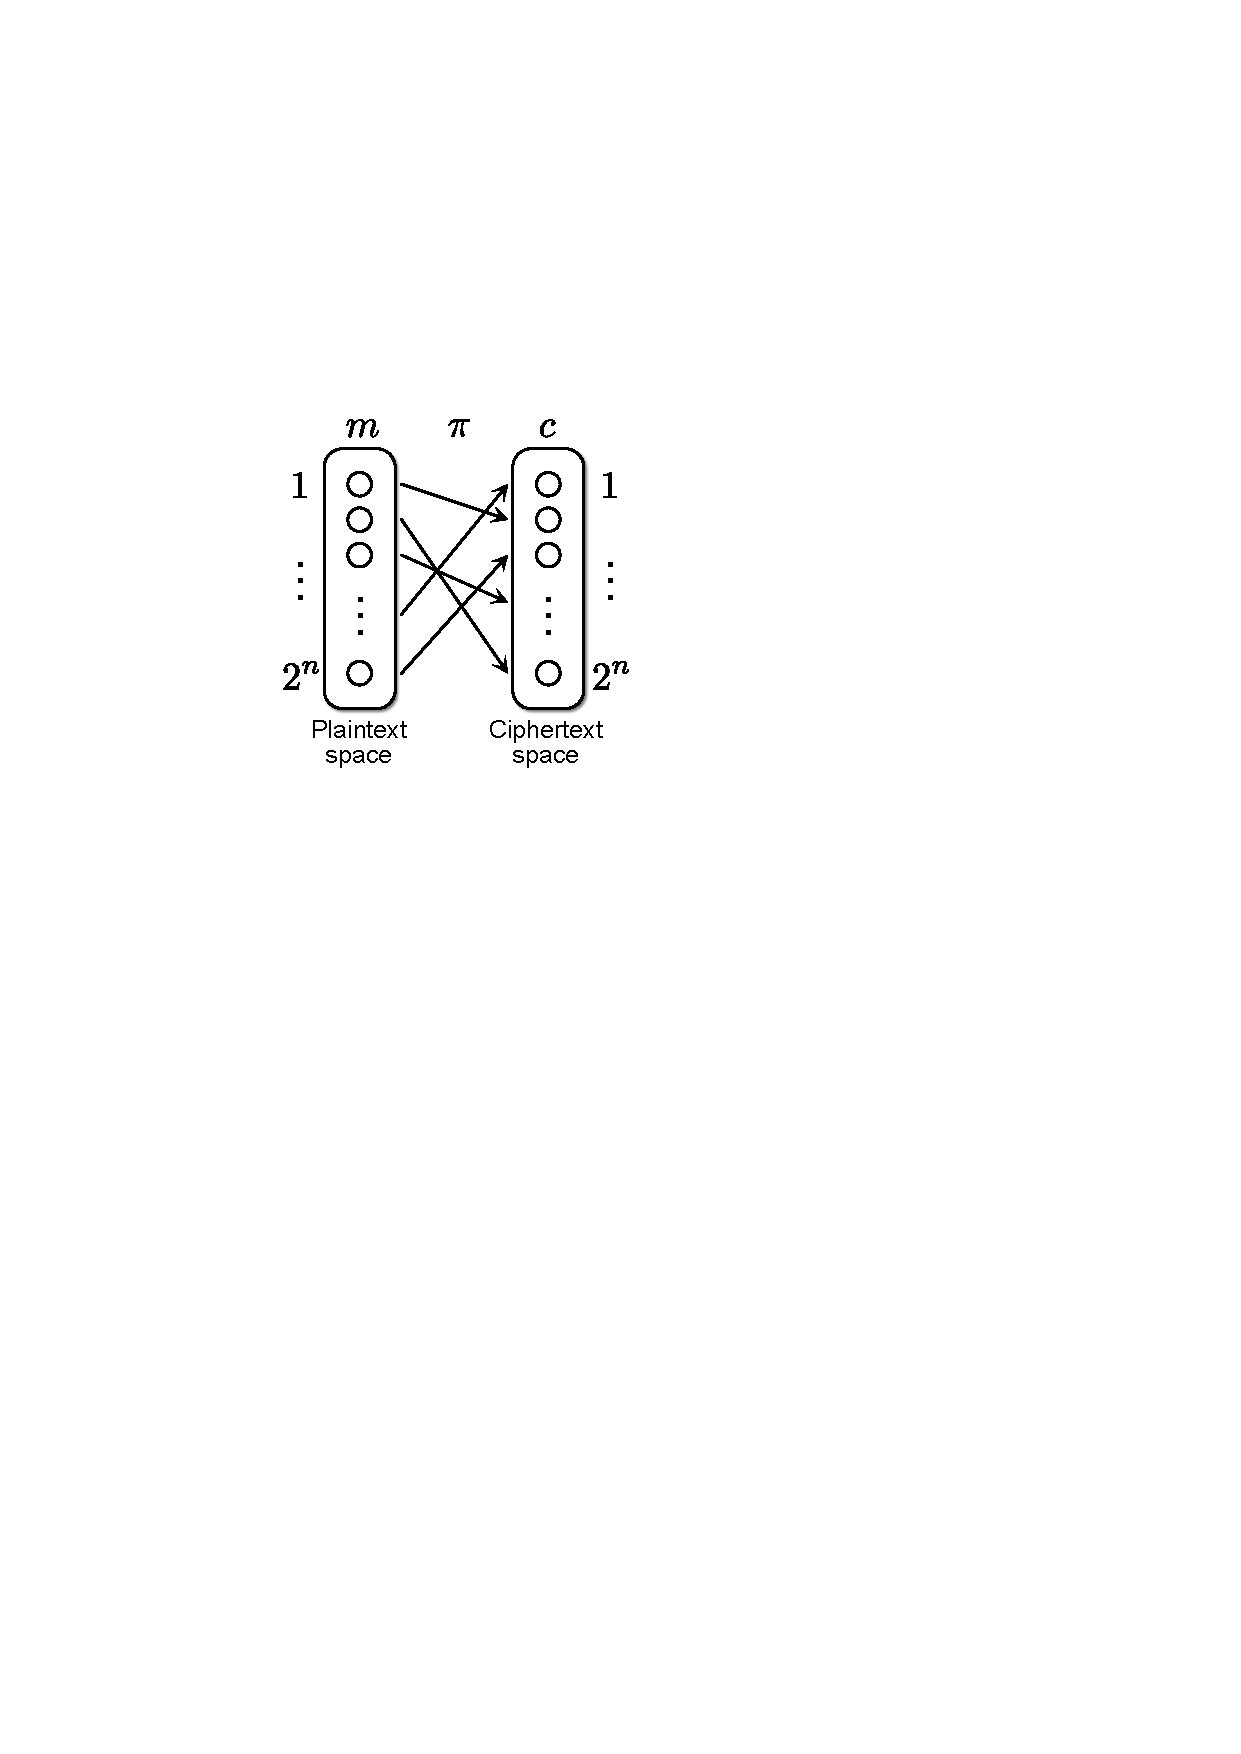
\includegraphics[width=0.5\columnwidth]{figures/block_cipher}
	\caption{Structure of a block cipher. For a block size of $n$ bits there are $2^n$ possible plaintexts, similarly for ciphertexts. Since every plaintext ($m$) must uniquely map to a distinct ciphertext ($c$), it follows via a pigeonholing argument that the encryption operation is effectively defined as a bijective map $\pi$ between the two spaces, such that $\vec{c}=\pi\cdot \vec{m}$.} \label{fig:block_cipher}	
\end{figure}

\subsubsection{Stream ciphers}

Stream ciphers act on data streams as opposed to blocks, with no inherent constraints on the size of the data. Here the data-stream is bitwise XORed with a pseudo-random sequence generated from the key and data-stream history, providing significant similarities with the one-time-pad (Sec.~\ref{one-time-pad-encryption}).

Although stream ciphers are useful for low-latency applications, they are less robust against errors than block ciphers. In a block cipher, an error within a plaintext (ciphertext) block will remain contained in the corresponding ciphertext (plaintext) block. In a stream cipher, on the other hand, any introduced errors will propagate indefinitely through the remainder of the stream owing to the intrinsic feedback loop, making error recovery challenging.

The structure of a stream cipher is shown in Fig.~\ref{fig:block_cipher}.

\begin{figure}[!htb]
	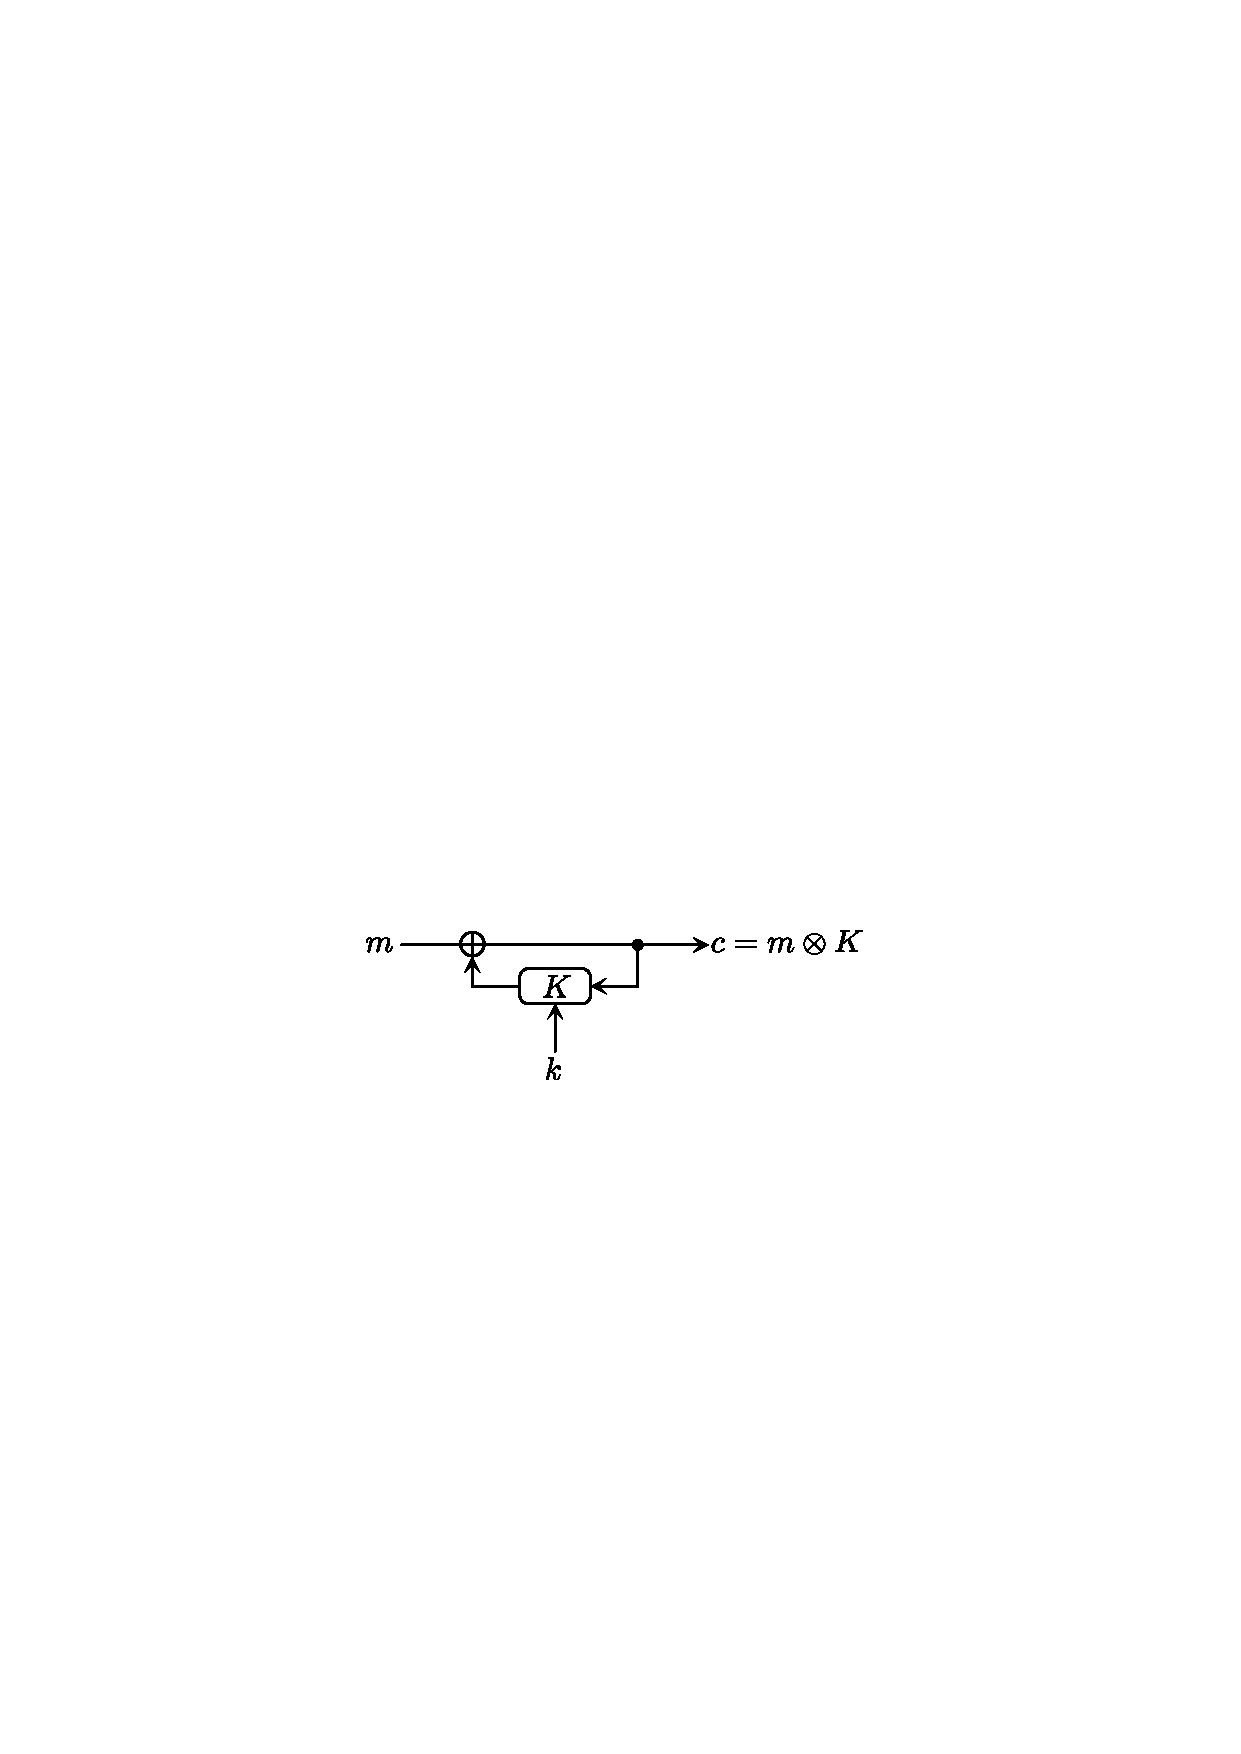
\includegraphics[width=0.8\columnwidth]{figures/stream_cipher}
	\caption{Structure of a stream cipher. A message stream $m$ is mapped to a ciphertext stream $c$ via XORing with a pseudorandom string $K$, $c=m\otimes K$. $K$ is derived as a function of the key $k$ and feedback from the previously encrypted output stream.} \label{fig:stream_cipher}	
\end{figure}

\subsubsection{One-time-pad encryption} \label{one-time-pad-encryption}

Of all the classical ciphers there is one and one only that exhibits perfect information-theoretic security, the one-time-pad (OTP) or Vernam cipher. The OTP, however, is an especially impractical symmetric cipher that requires a key as long as the message which can only be used once (hence the name).

Mathematically, the encryption and decryption operations are trivial to implement, simply bitwise XOR operations applied between the message and key to yield the ciphertext,
\begin{align}
	c = m \oplus k,
\end{align}
or between ciphertext and key to recover the message,
\begin{align}
	m = c \oplus k.
\end{align}
Note that the encryption and decryption operations are symmetric since,
\begin{align}
	{\tt enc}_k(m) = {\tt dec}_k(m) = m \oplus k.
\end{align}

But why is this extremely simple cipher perfectly secure? Consider trying to perform a brute-force attack against a ciphertext $c$ by exhaustively trying out every possible key $k_i$. Each $k_i$ will decrypt $c$ to a unique message, 
\begin{align}
    m_i = c \oplus k_i,
\end{align}
meaning that every message of the given length is an equally likely outcome, with no statistical biases or structures of any kind to exploit. If your message is $n$-bits in length, there are $2^n$ possible choices of key, which uniquely reproduce all $2^n$ possible $n$-bit messages.

So the most we can learn is the message's length, which admittedly isn't nothing. If a military general is giving orders, the difference in length between the messages `yes' and `no' is significant, although this is something easily obscured by padding messages to form fixed-length packets.

The non-reusability of the key stems from the fact that for two ciphertexts encoded with the same key we have,
\begin{align}
	c_1\oplus c_2 = (m_1\oplus k)\oplus(m_2\oplus k) = m_1 \oplus m_2,
\end{align}
which is the XOR of the two unencrypted plaintext messages, lending itself to a trivial frequency analysis attack.

Despite the impracticality of the one-time-pad cipher, it has found its place in history. During the Cold War, it was known that diplomats would carry suitcases full of OTP keys between embassies, which after being used were destroyed. However, this isn't an approach likely to find widespread utility for pragmatic reasons, unless we find a more practical way of sharing random bit-strings, to be discussed in Sec.~\ref{quantum-key-distribution-qkd}.

\subsection{Public-key cryptography} \label{public-key-cryptography}

The other form of cryptography is public-key cryptography, also known as \emph{asymmetric} cryptography since unlike symmetric cryptography different keys are used for encryption and decryption, known as the public ($k_{\tt pub}$) and private ($k_{\tt priv}$) keys (collectively a key-pair). The public key can only be used for encryption, and the private key only for decryption, yielding the following properties, 
\begin{align}
{\tt enc}_{k_{\tt pub}}(m) &\to c, \nonumber\\
{\tt dec}_{k_{\tt priv}}(c) &\to m, \nonumber\\
{\tt dec}_{k_{\tt priv}} \circ {\tt enc}_{k_{\tt pub}}(m) &= m.
\end{align}

As the name suggests, the public key can be made public while the private key must be kept private. Importantly, it should not be computationally possible to determine $k_{\tt priv}$ from $k_{\tt pub}$, for the obvious reason that if that were possible everyone could decrypt our messages using the published public key.

This property arises through the use of \emph{trapdoor functions} --- functions that are easy to perform in one direction, but hard to invert in the other. If the private key and public keys are related via such a function it means determining the private key from the public key is extremely difficult, whereas the person possessing the private key can easily manufacture the associated public key.

Public-key cryptography overcomes the impracticality we observed with private-key cryptography. We don't need any \emph{a priori} secrecy to share private keys. Instead, we can do everything over public channels.

Public-key ciphers do, however, have some disadvantages. Firstly, they do not preserve message length during encryption, instead inducing significant overheads in message size. Second, they tend to be algorithmically slower than symmetric ciphers. And thirdly, both of the most popular public-key cryptosystems we use today (RSA and ECC) are vulnerable to quantum attacks via variations on Shor's algorithm (Sec.~\ref{shors-algorithm}).

\subsubsection{RSA (Rivest-Shamir-Adleman)} \label{rsa-rivestshamiradleman}

The RSA public-key cryptosystem \cite{bib:RSA}, named after its inventors, was the first well-known public-key cryptosystem. Here the underlying trapdoor function is integer multiplication, specifically the multiplication of large prime numbers. Multiplication is a straightforward thing to do, even for very large numbers. Taking two prime numbers $p$ and $q$ it is easy to calculate $n=pq$. However, the inverse function of factorisation turns out to be far more complex, and indeed prohibitive via all known classical approaches --- given $n=pq$ it is hard to find $p$ and $q$. This is an example of an \textbf{NP} problem not believed to reside in \textbf{P}.

The best-known classical algorithm for factorising large integers is the general number field sieve, which exhibits time complexity,
\begin{align}
	O(e^{c (\log n)^{1/3}(\log\log n)^{2/3}}),
\end{align}
for an integer consisting of $\lfloor\log_2 n\rfloor+1$ bits. For large numbers, this scaling is highly inefficient. For quantum computers, the story is different, as discussed in Sec.~\ref{shors-algorithm} on Shor's algorithm.

In addition to encryption, by reversing the roles of the private and public keys RSA also lends itself to digital signatures.

The disadvantage of RSA public-key cryptography compared to private-key cryptography is twofold:
\begin{itemize}
	\item RSA keys are significantly larger than contemporary private keys. While private keys are often chosen to be 128 or 256 bits in length, RSA keys are typically chosen to be 2,048 to 4,096 bits in length.
	\item Private key encryption algorithms like AES create ciphertext the same length as the plaintext. RSA on the other hand creates ciphertext messages significantly longer than the plaintext.
	\item The RSA algorithm is far more compute-intensive than, say, AES. To address the above problems, RSA is typically used in hybrid form with AES, where RSA public-key cryptography is used to exchange an AES private key, after which all encryption is conducted via the more efficient AES.
\end{itemize}

It should be noted that it has not been \emph{proven} that integer factorisation is a hard problem. Rather, it has been extensively studied and the best-known algorithms are very computationally hard. This is therefore a not-so-strong example of computational security. It cannot be ruled out that better algorithms will be found or that the problem ends up being proven to not be classically hard at all.

\subsubsection{Elliptic-curve cryptography (ECC)} \label{elliptic-curve-cryptography-ecc}

Elliptic-curve cryptography (ECC) is a more recent approach to public-key cryptography, which like RSA can be used both for encryption or digital signatures. Here the trapdoor function relates to the difficulty of finding the discrete logarithm of a particular group.

Specifically, for some group $G$ where $a,b\in G$ and
\begin{align}
a=b^k,
\end{align}
we can write,
\begin{align}
k=\log_b a,
\end{align}
which reads $k$ is the discrete logarithm of $a$ to the base $b$. While not believed to be classically efficient in general (depending on the group $G$), the discrete logarithm problem can be solved efficiently using a variation of Shor's algorithm on quantum computers (Sec.~\ref{shors-algorithm}).

The primary advantage of ECC over RSA relates to efficiency. For the same level of security, ECC keys can be substantially shorter than RSA keys. The ECC algorithm is also more computationally efficient.

\subsection{Key exchange protocols} \label{key-exchange-protocols}

Given that public-key cryptography induces overheads in message size that symmetric ciphers such as AES-256 don't, we can hybridise these approaches to get the best of both worlds.

Rather than using public-key cryptography to encrypt our messages directly, we can instead use it to exchange private keys, which are subsequently used in a symmetric cipher. Such hybrid approaches are the norm, with the Diffie-Hellman algorithm \cite{bib:DiffieHellman} and its subsequent evolutionary variants being widely used.

A conceptual model for using public-key cryptography for key exchange could be described as follows (see Figs.~\ref{fig:KEM_1} \& \ref{fig:KEM_2}):
\begin{itemize}
	\item Alice and Bob share public keys.
	\item They both prepare independent random secret keys ($s_A$ and $s_B$).
	\item Using one another's public keys they exchange secrets.
	\item Now both parties possess both secrets, which can be combined to make a unified shared secret,
		\begin{align}
			s=s_A\oplus s_B.
		\end{align}
\end{itemize}
This isn't exactly how Diffie-Hellmann works, but is conceptually similar.

\begin{figure}[!htb]
	\centering
	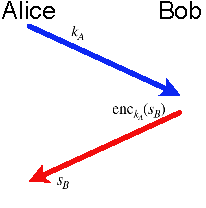
\includegraphics[width=0.75\columnwidth]{figures/Key_exchange_one_way}
	\caption{Two-party key exchange protocol using public-key cryptography. Both parties make their public keys known. Bob uses Alice's public key to securely send her a secret key. (Blue denotes public information, red denotes encrypted information)} \label{fig:KEM_1}
\end{figure}

\begin{figure}[!htb]
	\centering
	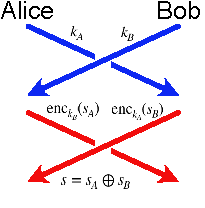
\includegraphics[width=0.75\columnwidth]{figures/Key_exchange_two_ways}
	\caption{Two-party key exchange protocol using public-key cryptography. Both parties make their public keys known, which are used to communicate random secrets with one another. These are combined to yield the master key, which is only compromised if channels in both directions are compromised, making man-in-the-middle attacks more challenging than in Fig.~\ref{fig:KEM_1}. (Blue denotes public information, red denotes encrypted information)} \label{fig:KEM_2}
\end{figure}

These are referred to as \emph{key encapsulation mechanisms} (KEMs) since the private key used for the subsequent symmetric cipher is encapsulated in the message of the asymmetric cipher. Note that in the second model, the shared secret is only compromised if the communication of \emph{both} secrets is compromised, making a man-in-the-middle attack more challenging.

\subsection{Hash functions} \label{hash-functions}

An extremely important class of cryptographic primitives is \emph{hash functions}. A hash function takes an input string $m$ of arbitrary length, and outputs a fixed-length \emph{hash} $h$ (also known as a \emph{checksum} or \emph{digest}),
\begin{align}
	{\tt hash}(m)\to h.
\end{align}

There are several properties we would like functions to exhibit to specifically call them \emph{hash functions}:
\begin{itemize}
	\item Pseudo-randomness: the output to a hash function should appear statistically random and unstructured. Changing a single bit on the input should on average flip half the bits on the output. If you were to use a clock signal as the input, you would have a very good random number generator (this is often exactly how it's done).
	\item Fast to compute: this is a practical issue since we will often want to create checksums for very large pieces of data.
	\item Uniform output probability distribution: averaged over all inputs, all outputs should be equally likely.
\end{itemize}

The use of hash functions is widespread not only within the field of cryptography. For example, checksums can be used for error detection --- when we transmit data we simultaneously transmit its checksum for verification by the recipient.

For cryptographic applications, we desire our hash functions to exhibit some additional properties from which they inherit their cryptographic utility. This leads to the notion of \emph{cryptographic hash functions}, which observe the following additional properties:
\begin{itemize}
	\item \textbf{Pre-image resistance}: for a given hash $h$ it should be computationally difficult to find an input message $m$ that hashes to that value such that ${\tt hash}(m)\to h$.
	\item \textbf{Second pre-image resistance} (aka weak collision resistance): if some message $m_1$ hashes to some value, it should be computationally difficult to find another message $m_2$ that hashes to the same value, such that ${\tt hash}(m_1)={\tt hash}(m_2)$.
	\item \textbf{Collision resistance} (aka strong collision resistance): generalising from the notion of second pre-image resistance, it should be difficult to find \emph{any} two messages that hash to the same value such that ${\tt hash}(m_1)={\tt hash}(m_2)$. When such a pair of messages are found (which must necessarily exist), they are referred to as a \emph{hash collision}.
\end{itemize}

The best-known class of cryptographic hash functions used today is the SHA-2 family of hash functions. This contains several hash functions producing hashes of different lengths, after which they are named. For example, SHA-256 generates a 256-bit hash function.

\emph{Inverse hashing} is the problem of breaking the pre-image resistance of hash functions, finding an input string that hashes to a specified output string,
\begin{align}
	{\tt hash}^{-1}(h)\to m.
\end{align}
For a cryptographically strong hash function, brute-force ought to be the best one can do, which has exponential time complexity.

\subsection{Authentication}

An essential cryptographic primitive is authentication, whereby someone wishes to prove their identity to another party or sign a document to prove that they wrote it, so-called \emph{digital signatures}.

\subsubsection{Authentication using shared secrets} \label{authentication-using-shared-secrets}

If two parties have a pre-existing shared secret (i.e a secret private key) and are confident they are the only ones in possession of it, it becomes trivial to implement a two-party authentication scheme (or signature) using cryptographic hash functions, specifically by exploiting the pre-image resistance property. This can be used to both confirm someone's identity or to sign messages.

\paragraph{Message authentication}

To transmit an authenticated message $m$, Alice transmits to Bob,
\begin{align}
	{\tt auth}(m) = m|{\tt hash}(s|m).
\end{align}
That is, she transmits a message along with a hash of the message and private key. Upon receiving $m$, Bob calculates ${\tt hash}(s|m)$ and checks for consistency between what he calculated and what he received.

This approach not only authenticates the message, but simultaneously serves to detect transmission errors in $m$ by acting as a message checksum, as any errors would change the associated hash.

This technique closely resembles the HMAC (hash-based message authentication code) protocol. The advantage of this approach to authentication lies primarily in efficiency. Public-key signatures (Sec.~\ref{ref:public_key_dig_sig}) are relatively computationally intensive, whereas hash functions are by design highly computationally efficient to evaluate. Combining the two, public-key cryptography could be used for the exchange of a secret key, subsequently utilised by the more efficient HMAC.

\paragraph{User authentication}

Suppose two users in possession of a shared secret key wish to authenticate a channel so as to be convinced they are speaking to one another. This can be achieved using message authentication as a primitive. If Alice wishes to confirm that she is speaking to Bob, she first prepares and signs a random message $m$, sending,
\begin{align}
	{\tt auth}(m) = m|{\tt hash}(s|m).
\end{align}
Bob first calculates ${\tt hash}(s|m)$ to confirm the integrity of the received $m$. If successful, he responds by replying with,
\begin{align}
	{\tt auth}(m|m) = m|m|{\tt hash}(s|m|m),
\end{align}
which Alice is able to evaluate for consistency. Here we have opted for Bob to transmit ${\tt hash}(s|m|m)$ since this creates a hash proving that Bob is in possession of Both $m$ and $s$, but which is distinct from the already transmitted ${\tt hash}(s|m)$. Note that ${\tt hash}(s|m)$ and ${\tt hash}(s|m|m)$ cannot be inferred from one another without knowing $s$.

% For a given message $m$ and shared secret $s$, a signature for $s$ can be made by hashing the concatenated message and secret key,
% \begin{align}
% 	{\tt sig}={\tt hash}(s|m),
% \end{align}
% where the vertical bar represents string concatenation. The other party, also in possession of the shared secret $s$ can easily reevaluate ${\tt sig}$ upon receiving the message $m$. It can easily be seen that a fraudulent signature cannot be made by anyone not in possession of $s$, but additionally the signature can only be verified by someone in possession of $s$, effectively limiting this to two-party scenarios.

% For two parties to confirm that they are speaking to one another the protocol for authentication could proceed as follows:
% \begin{itemize}
% 	\item Alice and Bob both prepare random messages, $m_A$ and $m_B$.
% 	\item They communicate these messages via the channel they want to authenticate.
% 	\item They both calculate \mbox{${\tt sig}_A={\tt hash}(s|m_A)$} and \mbox{${\tt sig}_B={\tt hash}(s|m_B)$} which are shared via the channel.
% 	\item If the values for ${\tt sig}_A$ and ${\tt sig}_B$ calculated by Alice and Bob are consistent with the ones sent by the other it implies the two parties must have possessed the shared secret $s$ and are hence who they say they are.
% 	\item Anyone else possessing $s$ could spoof being the other party and perform a man-in-the-middle attack.
% \end{itemize}

%While this scheme is very robust if the underlying hash function satisfies the pre-image resistance requirement, it relies on a pre-existing shared secret key, which must be shared via other means.

%highly impractical given the requirement that both parties must find the means to share a secret key a priori.

In a multi-user environment with $n$ users, all of whom wish to be able to sign messages with one another, this approach requires on the order of $O(n^2)$ secret keys.

\subsubsection{Public-key digital signatures} \label{ref:public_key_dig_sig}

Despite being very secure, inheriting their security from the pre-image resistance of hash functions, authentication using shared secrets requires first sharing a secret key. Ideally we would like a system with properties akin to public-key cryptography, whereby someone can make available a public key that others can use to verify a signature made with the associated private key. Specifically, we want the following mathematical properties,
\begin{align}
{\tt sign}_{k_{\tt priv}}(m) &\to s, \nonumber\\
{\tt verify}_{k_{\tt pub}}(s) &\to m, \nonumber\\
{\tt verify}_{k_{\tt pub}} \circ {\tt sign}_{k_{\tt priv}}(m) &= m,
\end{align}
where $m$ is the message, $s$ is the signature, and $k_{\tt priv}$ cannot be efficiently determined from $k_{\tt pub}$.

Interestingly, both the RSA and ECC encryption schemes can be used for exactly this purpose, simply by interchanging the roles of the public and private keys. A message is signed by applying RSA/ECC using what is now the private key, which can be decrypted and hence verified (but not forged) using what is now the public key. Now someone producing the keypair has the ability to publish a key that can be used for verification but not signing, whilst keeping the one used for signing secret, which cannot be efficiently determined from one another.

This ability to interchange the roles of keys to use RSA/ECC for digital signatures is more fortuitous than by design, and not something that need hold in general for asymmetric ciphers. Rather, it is specific to RSA/ECC.

As discussed in Sec.~\ref{authentication-using-shared-secrets}, when using shared secrets for authentication, $O(n^2)$ secret keys need to be exchanged (one for each user-pair), highly impractical for many applications. Contrast this with reusable public-key digital signatures in which there need only be $n$ public-keys (one for each user), which can be communicated via public channels with no need for any secret exchanges. This makes public-key digital signatures far more versatile and practical than authentication using shared secrets.

However, in the same way that RSA/ECC encryption may be compromised using Shor's algorithm, so too can RSA/ECC digital signatures. In this instance, a successful Shor attack would allow messages to be fraudulently signed as opposed to decrypted.

In the quantum era, where Shor attacks are viable, it will therefore be necessary to transition to post-quantum digital signatures, to be discussed in Sec.~\ref{post-quantum-cryptography-pqc}. In the same way that quantum cryptography only enables private-key cryptography, there are no known quantum digital signature schemes satisfying our desired properties.

\subsection{One-time passwords (OTP)}

When manually logging into websites using a password, many sites now provide the option or require the use of two-factor authentication (2FA), where in addition to the password some other secondary mechanism is used to confirm identity. These are commonly implemented using one-time passwords (OTPs). In some instances these are communicated by SMS text messages or email. In others it is implemented using time-based one-time passwords (TOTPs), which we describe here.

When configuring an account, in addition to the primary password, a shared secret is established between the client and server, using conventional KEMs, as described previously. The shared secret is held on the client's device but not directly visible to the user. The TOTP is calculated by hashing the shared secret with a timestamp, such that the TOTP is constantly evolving as a function of time, but in a way which does not disclose the shared secret nor the TOTP at other times. Specifically,
\begin{align}
\mathtt{TOTP} = \mathtt{hash}(k|t),	
\end{align}
where $k$ is the shared secret key, and $t$ is a timestamp rounded off to some pre-agreed increment. Here the hash function is typically chosen to produce a short hash of say six decimal digits or so for the purposes of practicality.

Note that via the pre-image resistance of the hash function, establishing the shared secret key $k$ from the TOTP is not viable. Since the TOTP is a hash and only used once, it needn't be encrypted.

Since TOTPs rely on the establishment of a secret key, they could in principle be implemented using quantum key distribution, described in Sec.~\ref{quantum-key-distribution-qkd}.

\subsection{Ratchets} \label{ratchets}

The risk of man-in-the-middle attacks is one that is difficult to rule out. But despite being impossible to discount, we can make life harder for them by giving them more work to do. Suppose the attacker didn't just have to perform an intercept-resend attack once to read a single message, but instead was required to spoof all messages from the message history. This would require a much more consistent and committed effort by the adversary. This introduces the notion of \emph{ratchets}, whereby keys at all points in time must be compromised to break security (see Fig.~\ref{fig:ratchet}).

The idea of ratchets has been popularised by the Signal protocol \cite{bib:SignalProtocol}, used in the Signal messaging app. The goal of this technique is to both improve security and provide so-called \emph{forward secrecy} and \emph{backward secrecy}:
\begin{itemize}	
	\item Forward secrecy: when a user stops participating in a communication (i.e they are denied future session keys) they are unable to decrypt future messages.
	\item Backward secrecy: compromising the current key does not unlock past messages or the present one if past keys are not also known.
\end{itemize}

The approach here is for communicating parties to hold a local \emph{state register} on their device. For every communication, a new key is exchanged. The session key actually used to encrypt the communication is obtained by hashing together the state register and the newly exchanged key. The register is then updated to hold this session key for the next round,
\begin{align}
	s_n=\texttt{hash}(k_n|s_{n-1})
\end{align}

\begin{figure}[!htb]
	\centering
	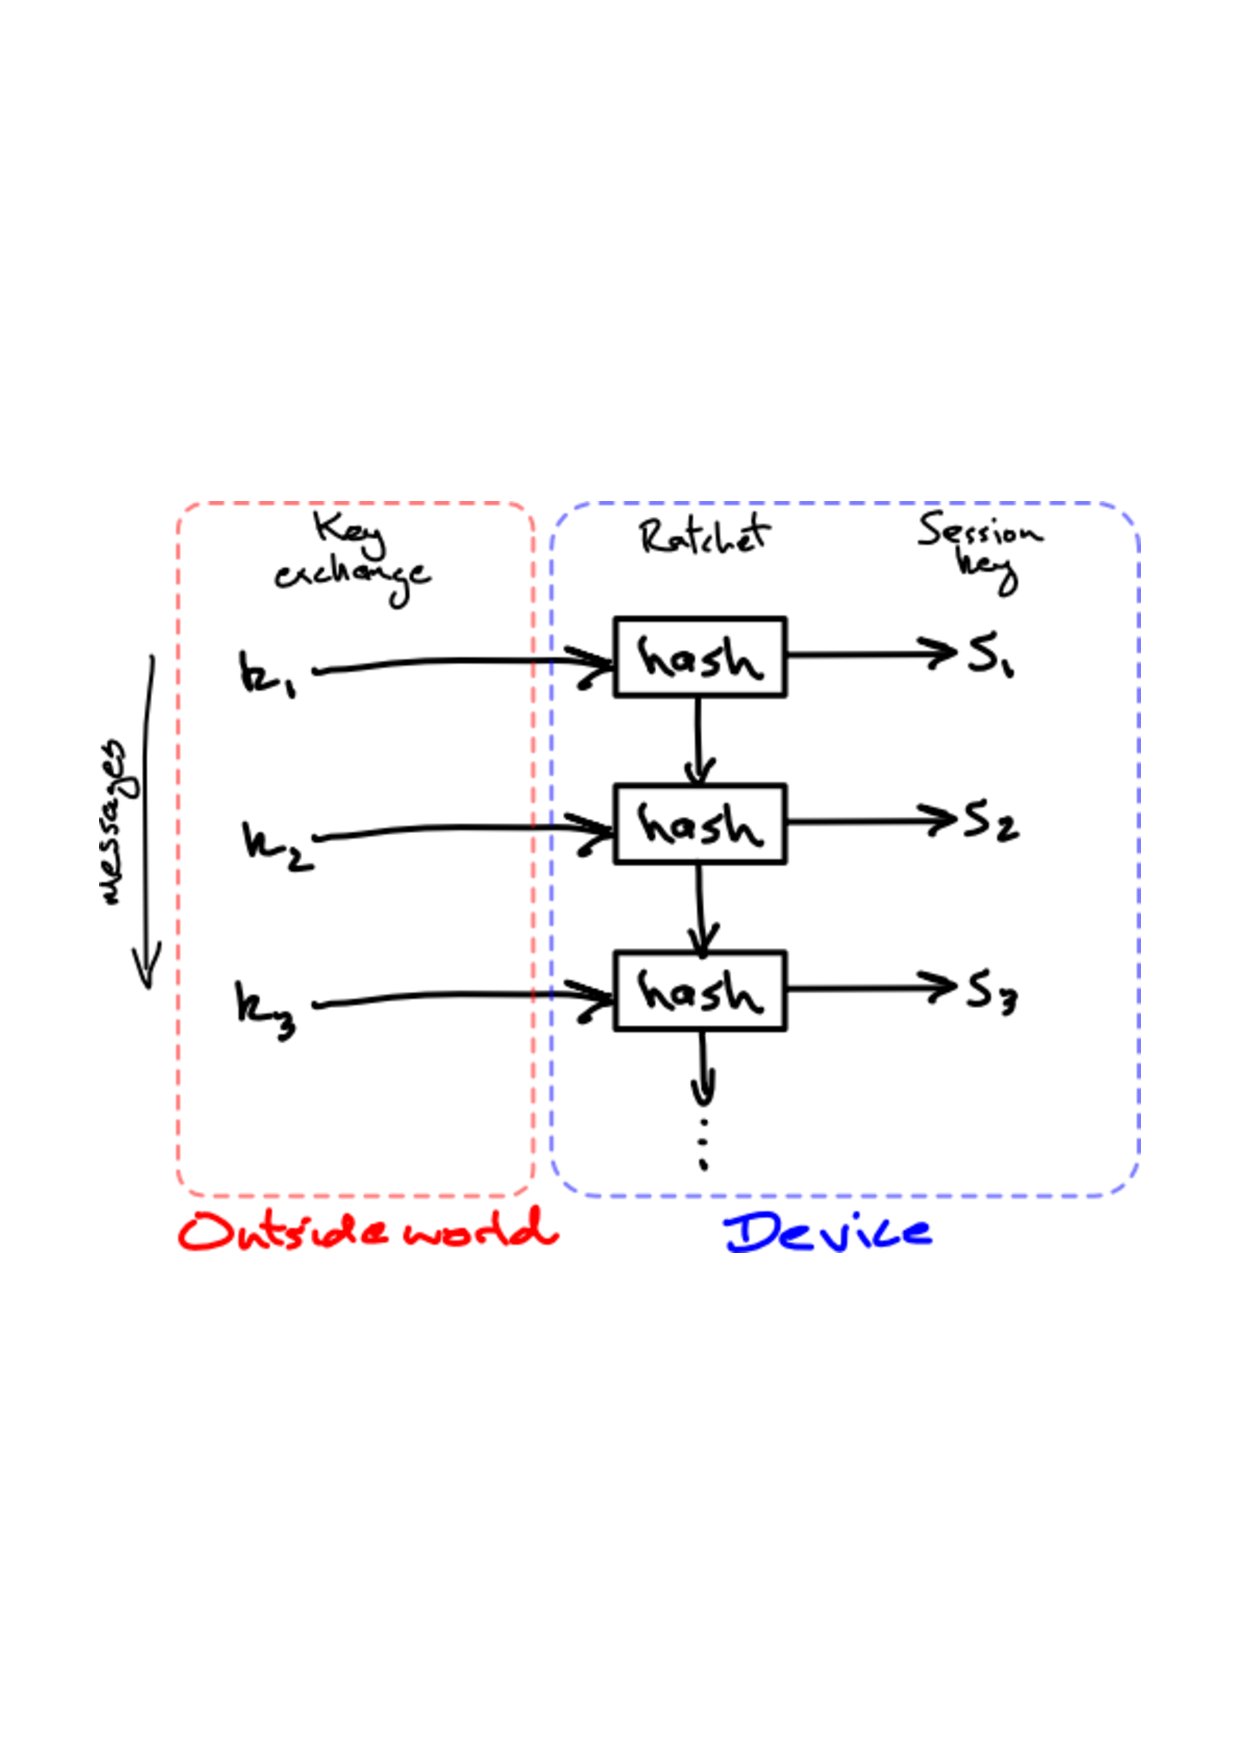
\includegraphics[width=\columnwidth]{figures/Ratchet}
	\caption{A simple ratchet mechanism whereby the current session key is derived from a hash of the most recently exchanged key and the previous session key. This mechanism provides both forward and backward secrecy, and ensures that a session key can only be compromised if all previously exchanged keys were compromised.} \label{fig:ratchet}
\end{figure}

From the diagram above it is evident via the pre-image resistance of the hash function, that intercepting some key $k_n$ does not allow the session key $s_n$ to be determined unless the state register is known, which is a function of all previous session keys. That is, all exchanged private keys must have been intercepted to determine the current session key. This provides our backward secrecy.

Similarly, if this were a group communication and a party stopped receiving newly exchanged keys, they would not be able to determine future session keys, thereby providing our forward secrecy.

The introduction of ratchets significantly complicates life for adversaries attempting to perform man-in-the-middle attacks and one of the reasons the Signal protocol is deemed so secure (see Fig.~\ref{fig:musk}).

\begin{figure}[!htb]
	\centering
	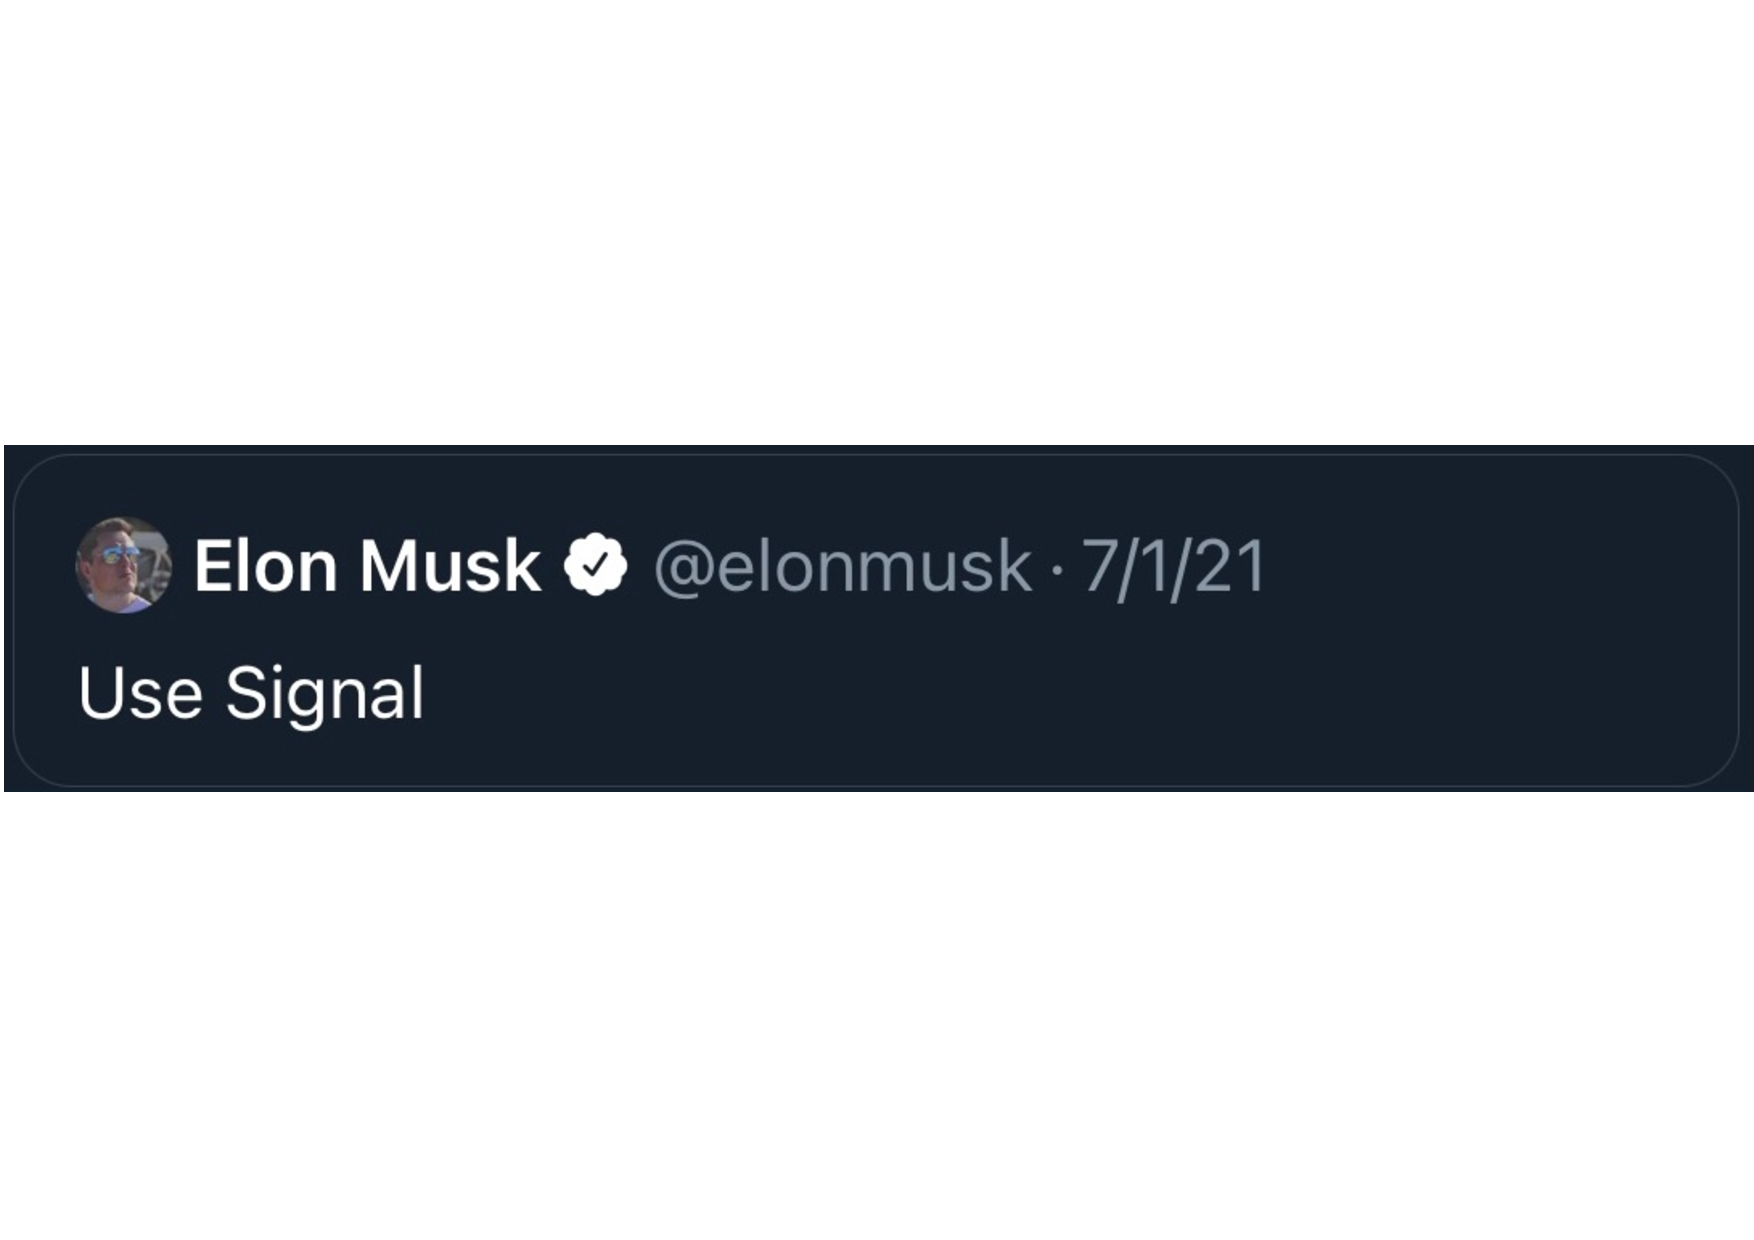
\includegraphics[width=\columnwidth]{figures/Musk}
	\caption{Elon Musk's views on the Signal messaging app.} \label{fig:musk}
\end{figure} 

\subsection{Zero-knowledge proofs (ZKPs)}

A \textit{zero-knowledge proof} (ZKP) is an interactive protocol between two parties --- a \textit{prover} Peggy, and a \textit{verifier} Victor --- where Peggy wishes to efficiently prove to Victor that she knows the solution to a problem, without actually revealing the solution. Thus, a ZKP can serve as a signature that a problem has been faithfully solved, without disclosing the solution.

ZKPs are useful in a number of cryptographic applications, most notably in authentication. In the case of classical computing, a variety of free software packages are available for compiling ZKPs for generic code. However, ZKPs become far more valuable in the case of cloud quantum computing, where there is an inherent complexity asymmetry between the client Victor (classical resources only) and the server Peggy (full quantum resources), whereby efficient ZKPs become a useful transactional tool during computational outsourcing. In a commercial context, a client can convince themselves that a server has actually performed an outsourced computation before finalising the transaction.

\subsubsection{Graph isomorphism}

A conceptually simple example for illustrating the operation of a ZKP protocol is the \textit{graph isomorphism problem}. Two graphs are \textit{isomorphic}, denoted \mbox{$G_1\sim G_2$}, if there exists a permutation \mbox{$\pi\in S_n$}\footnote{In group theory, $S_n$ denotes the symmetric group, the set of all permutations on $n$ elements, of which there are \mbox{$|S_n|=n!$} (the order of the group).} on their vertex labels that makes them equivalent, i.e \mbox{$G_1=\pi\cdot G_2$}\footnote{Here we have employed the operator notation that \mbox{$\pi\cdot G$} means `permutation $\pi$ applied to graph $G$'. Alternately, in matrix notation, where $\pi$ is a permutation matrix and $G$ is an adjacency matrix, this operation implies the matrix conjugation \mbox{$\pi\cdot G\cdot\pi^\top$}.}. The graph isomorphism problem is to find $\pi$ for arbitrary $G_1$ and $G_2$.

This problem is clearly contained in \textbf{NP}, since permuting vertices in graphs and directly comparing them are both computationally straightforward, making verification of the problem a polynomial-time affair. However, it is believed that explicitly determining the respective permutation is difficult in general. This is intuitively unsurprising, since for a graph with $n$ vertices, there are $n!$ possible permutations to consider (which is super-exponential), and therefore a na{\" i}ve brute-force approach would require $O(n!)$ comparisons in the worst-case\footnote{This is the worst-case scenario. In many special cases, knowledge of the underlying graph structure can simplify this enormously, yielding classically efficient runtimes.}. This problem is not believed to be contained in either \textbf{P} or \textbf{NP}-complete, and therefore presumed to be \textbf{NP}-intermediate.

\begin{figure}[!htpb]
	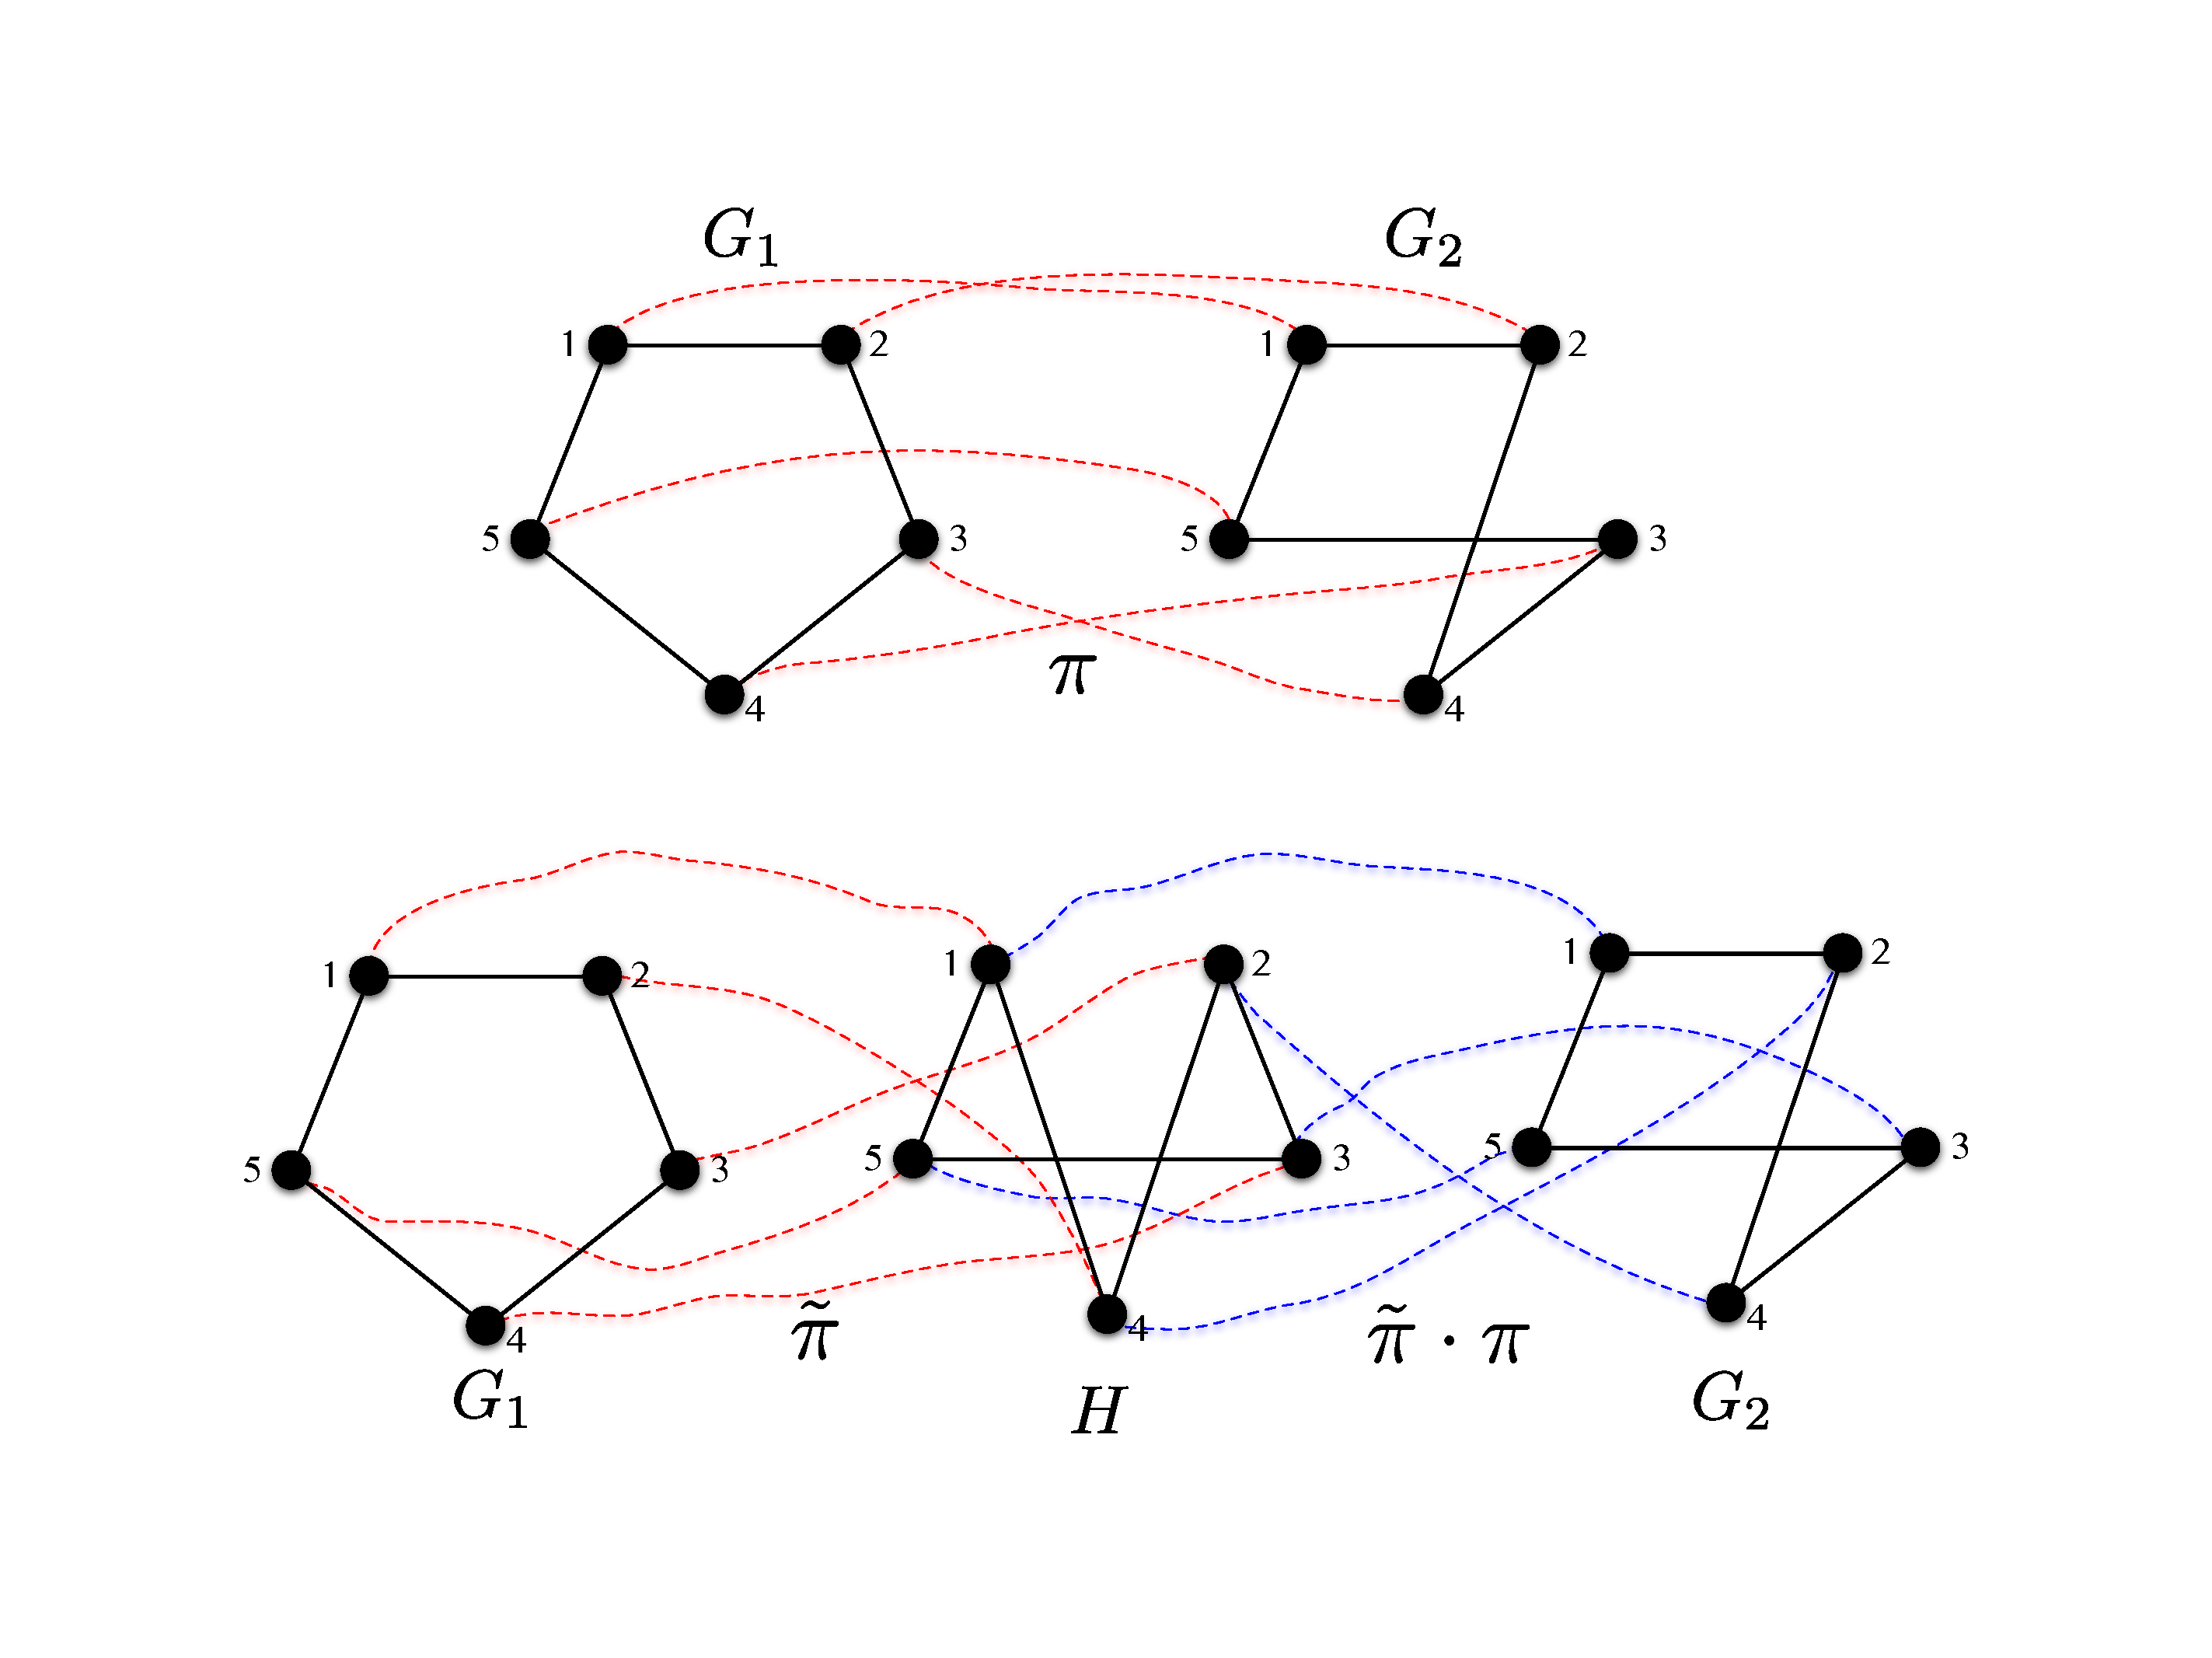
\includegraphics[width=\columnwidth]{figures/ZKP_graph_isomorphism}
    \caption{The isomorphisms \mbox{$G_1\sim G_2$} (top), and \mbox{$G_1\sim H\sim G_2$} (bottom). Coloured lines indicate the vertex relabelings associated with the respective isomorphisms. Knowing the isomorphisms \mbox{$G_1\sim H$} and \mbox{$G_2\sim H$} simultaneously implies knowledge of \mbox{$G_1\sim G_2$} via composition of the permutations. However, knowing only one of them does not, since $H$ is chosen randomly. By repeatedly, randomly proving knowledge of one of the two isomorphisms with $H$ we achieve asymptotic certainty that the prover must have known \mbox{$G_1\sim G_2$}, without actually revealing the associated permutation $\pi$.}\label{fig:ZKP_graph}
\end{figure}

In the example isomorphism presented in Fig.~\ref{fig:ZKP_graph}(top), the vertex permutation mapping $G_1$ to $G_2$ could be expressed in vector form as,
\begin{align}
\pi = \begin{pmatrix}
	1 \\
	2 \\
	3 \\
	4 \\
	5
\end{pmatrix}_{G_1} \to \begin{pmatrix}
	1 \\
	2 \\
	4 \\
	3 \\
	5
\end{pmatrix}_{G_2},
\end{align}
where indices denote vertex labels, or equivalently via the permutation matrix,
\begin{align}
\pi = \begin{pmatrix}
	1 & 0 & 0 & 0 & 0 \\
	0 & 1 & 0 & 0 & 0 \\
	0 & 0 & 0 & 1 & 0 \\
	0 & 0 & 1 & 0 & 0 \\
	0 & 0 & 0 & 0 & 1
\end{pmatrix}.
\end{align}

\begin{figure}[!htb]
\begin{mdframed}
\texttt{
function ZKP.GraphIsomorphism($G_1$, $G_2$):
\begin{enumerate}
	\item Graphs $G_1$ and $G_2$ are known to both verifier Victor and prover Peggy.
	\item Peggy knows the permutation $\pi$ for the isomorphism \mbox{$G_1\sim G_2$},
	\begin{align}
		G_1 = \pi \cdot G_2.
	\end{align}
	\item Peggy wishes to prove to Victor that she knows $\pi$, without disclosing what it is.
	\item Peggy chooses another random permutation $\tilde\pi$, and constructs the new permuted graph $H$,
	\begin{align}
		H &= {\tilde\pi}\cdot G_1\nonumber\\
		& = {\tilde\pi}\cdot \pi \cdot G_2.
	\end{align}
	\item Peggy shares $H$ with Victor, randomly isomorphic to both $G_1$ and $G_2$.
	\item Victor randomly (with probability \mbox{$p=1/2$}) asks Peggy to prove \textit{either} \mbox{$H\sim G_1$} or \mbox{$H\sim G_2$}.
	\item She accordingly reveals either $\tilde\pi$ or \mbox{$\tilde\pi\cdot\pi$} to Victor. He can now efficiently verify either \mbox{$H\sim G_1$} or \mbox{$H\sim G_2$} respectively, by performing the inverse permutation,
	\begin{align}
		G_1 &= {\tilde\pi}^{-1} \cdot H,\nonumber\\
		G_2 &= ({\tilde\pi}\cdot \pi)^{-1} \cdot H.
	\end{align}
	\item Victor is unable to determine $\pi$ from either scenario alone, but could were he to know \textit{both} isomorphisms simultaneously, since,
	\begin{align}
		\pi = {\tilde\pi}^{-1}\cdot (\tilde\pi\cdot\pi).
	\end{align}
	\item The above is repeated $n$ times. Each time, Peggy chooses a new random $\tilde\pi$.
	\item If Peggy does not actually know $\pi$, the probability of fraudulently passing this test $n$ times is,
	\begin{align}
		P_\text{deceive} = \frac{1}{2^n}	.
	\end{align}
	\item With confidence \mbox{$1-P_\text{deceive}$}, Victor knows that Peggy knows $\pi$, without knowing it himself.
	\item $\Box$
\end{enumerate}}
\end{mdframed}
\caption{A zero-knowledge proof for the graph isomorphism problem. Victor (verifier) provides two graphs to Peggy (prover), who can demonstrate with asymptotic certainty that she knows their isomorphism, without disclosing the associated permutation relating them.} \label{alg:ZKP_graph}
\end{figure}

To provide a ZKP for this, Peggy's goal is to prove that she knows $\pi$, without explicitly revealing it. An efficient, randomised, classical ZKP protocol for achieving this is provided in Fig.~\ref{alg:ZKP_graph}, and a specific example illustrated in Fig.~\ref{fig:ZKP_graph}. The key underlying principle here is to obscure $\pi$ through randomisation, whereby instead of directly proving knowledge of $\pi$, it is implied via multiple proofs of isomorphisms with intermediate random graphs.

\subsubsection{Hash functions}

Hash functions can be used to prove knowledge of a piece of data. If Alice and Bob both possess data $x$ then Alice can prove to Bob that she knows $x$ by revealing,
\begin{align}
y=\texttt{hash}(x).
\end{align}
This acts as a signature for $x$ from which $x$ itself cannot be determined owing to the pre-image resistance of the hash function.

This can additionally be used in a different context where Alice wishes to provide a public proof that she knows $x$ now, but doesn't wish to disclose $x$ itself until later. When at a later point in time she does reveal $x$, its previously published hash proves retrospectively that she knew it at the time of publishing $y$. This is sometimes referred to as \emph{commitment} and an important primitive especially in blockchain implementations.

By combining this technique with a digital signature scheme, if Alice signs the hash at the time of publication this additionally serves to prove her identity as the one who published it.

\subsubsection{Digital signatures}

Digital signatures on their own are also a form of ZKP, where identity is being proven. Since the private and public keys forming the key-pair are related by a trapdoor function, providing a digital signature (which can be verified using the public key) provides proof of ownership of the associated private key (which represents the user's identity and should be kept secret).